\documentclass[11pt]{article}
\usepackage[T1]{fontenc}
\usepackage[utf8]{inputenc}
\usepackage{lmodern}
\usepackage[margin=1in]{geometry}
\usepackage{parskip}
\usepackage{booktabs}
\usepackage{enumitem}
\usepackage{graphicx}
\usepackage{xcolor}
\usepackage[most]{tcolorbox}
\tcbuselibrary{skins,breakable}
\usepackage[colorlinks=true, linkcolor=blue!55!black, urlcolor=blue!55!black]{hyperref}
\setlist{itemsep=2pt, topsep=3pt}
\definecolor{accent}{RGB}{31,78,120}
\newtcolorbox{infobox}[1][]{colback={rgb,255:red,240;green,244;blue,248}, colframe={rgb,255:red,60;green,90;blue,130}, boxrule=0.8pt, arc=2pt, #1}
\newtcolorbox{warnbox}[1][]{colback={rgb,255:red,250;green,240;blue,238}, colframe={rgb,255:red,150;green,60;blue,50}, boxrule=0.8pt, arc=2pt, #1}

\title{\vspace{-1.2cm}\textbf{Rating Migration and Default Probability Under Stress}\\ \large A preregistered study on S\&P issuer ratings, 1985 to 2016}
\author{Zaid Annigeri}
\date{November 2026}

\begin{document}
\maketitle

\begin{infobox}
\textbf{Summary.} I estimate one-year rating transition matrices from 702,168 monthly S\&P issuer ratings, fit a one-factor credit-cycle index, link it to macro data, and test the link out of time. The cycle index is real: its worst years are 2002, 2001 and 2009. The macro link is not robust: it explains 82\% of the index in sample but predicts 2008 to 2016 default rates worse than a plain long-run average. The severely adverse projection is therefore reported as an extrapolation, not a forecast. Hypotheses were fixed before any model was fitted, and the failed one is reported.
\end{infobox}

\section{Question and hypotheses}

How do corporate default and downgrade probabilities move with the credit cycle, and what does a severely adverse scenario imply for them? Three hypotheses were written down before estimation (\texttt{PREREGISTRATION.md}):

\begin{itemize}
\item \textbf{H1.} Speculative-grade default rates peak in 1990-91, 2001-02 and 2009, and the cycle index is lowest in those years.
\item \textbf{H2.} A macro-linked model predicts 2008 to 2016 speculative-grade default rates with lower error than the through-the-cycle average.
\item \textbf{H3.} Under the severely adverse scenario the projected speculative-grade default rate is at least double its average.
\end{itemize}

\section{Data}

S\&P long-term issuer ratings from Compustat, monthly, 5,972 issuers. Modifiers are merged into letter grades, CCC+ to C form one grade, and D and SD are default, which is absorbing. The file is usable from the December 1985 cohort, giving 56,869 issuer-years. Macro series (unemployment, real GDP, Baa and 10-year Treasury yields) are from FRED. The stress scenario is the Federal Reserve's 2025 supervisory severely adverse scenario.

\begin{warnbox}
\textbf{Data gaps.} Checked against S\&P's published U.S. speculative-grade default rates, the file agrees well from 1999 to 2016 (correlation 0.90, median ratio 0.92) but under-records defaults before 1999 (1991: 1.25\% against S\&P's 10.71\%) and partly in 2009 to 2014 (2009: 6.75\% against 11.79\%). Default thresholds therefore use the 1998 to 2006 cohorts only, and H1 cannot be tested for 1990-91.
\end{warnbox}

\section{Method}

\textbf{Transition matrices.} The cohort method takes issuers rated on 31 December and records their grade one year later; transitions to not-rated are removed and rows renormalised. The duration method estimates monthly transition intensities and exponentiates the generator matrix.

\textbf{Cycle index.} Each row of the average matrix is mapped to thresholds of a standard normal variable. In year $t$ an issuer's credit variable is $\sqrt{\rho}\,Z_t + \sqrt{1-\rho}\,\varepsilon$, so a single number $Z_t$ shifts every row at once. $Z_t$ is fitted by maximum likelihood for each year, and $\rho$ is set so that $Z_t$ has unit variance over the estimation window. To keep under-recorded early defaults from driving the index, default is merged with CCC for this fit.

\textbf{Macro link and test.} $Z_t$ is regressed on the change in unemployment, real GDP growth and the Baa minus 10-year Treasury spread, using transition years 1986 to 2007 only. For 2008 to 2016, $Z_t$ is predicted from macro data alone and converted to a speculative-grade default rate. The benchmark is the through-the-cycle average matrix.

\section{Results}

\begin{table}[h]
\centering\small
\begin{tabular}{lrrrrrrrr}
\toprule
From / to & AAA & AA & A & BBB & BB & B & CCC & D \\
\midrule
AAA & 92.60 & 6.46 & 0.59 & 0.12 & 0.24 & 0.00 & 0.00 & 0.00 \\
AA & 0.59 & 89.13 & 9.62 & 0.54 & 0.03 & 0.10 & 0.00 & 0.00 \\
A & 0.02 & 1.22 & 91.57 & 6.57 & 0.38 & 0.17 & 0.02 & 0.06 \\
BBB & 0.01 & 0.05 & 3.10 & 92.03 & 3.97 & 0.55 & 0.13 & 0.16 \\
BB & 0.00 & 0.02 & 0.06 & 5.59 & 85.58 & 7.49 & 0.67 & 0.58 \\
B & 0.01 & 0.02 & 0.09 & 0.29 & 7.31 & 83.19 & 5.53 & 3.55 \\
CCC & 0.00 & 0.00 & 0.18 & 0.09 & 1.41 & 17.18 & 57.44 & 23.70 \\
\bottomrule
\end{tabular}
\caption{Average one-year transition matrix, cohort method, 1985 to 2015 cohorts (\%).}
\end{table}

\textbf{Cohort against duration.} The two methods count almost the same defaults (706 and 705) but the duration matrix gives lower one-year default rates for BBB (0.05\% against 0.16\%), BB (0.31\% against 0.58\%) and B (2.77\% against 3.55\%), and a higher one for CCC (31.99\% against 23.70\%). The duration method assumes the next move depends only on the current grade. The gap is consistent with recently downgraded issuers defaulting faster than their grade implies; that was not tested here.

\textbf{H1: holds where it can be tested.} The asset correlation is $\rho = 0.027$. The lowest values of the index are 2002 ($-2.08$), 2001 ($-1.92$) and 2009 ($-1.79$).

\textbf{Macro regression.} $R^2 = 0.82$ with 22 observations. Only the Baa spread is significant (coefficient $-1.78$, $t = -7.8$); unemployment change ($t = -0.5$) and GDP growth ($t = 0.9$) are not.

\begin{figure}[h]
\centering
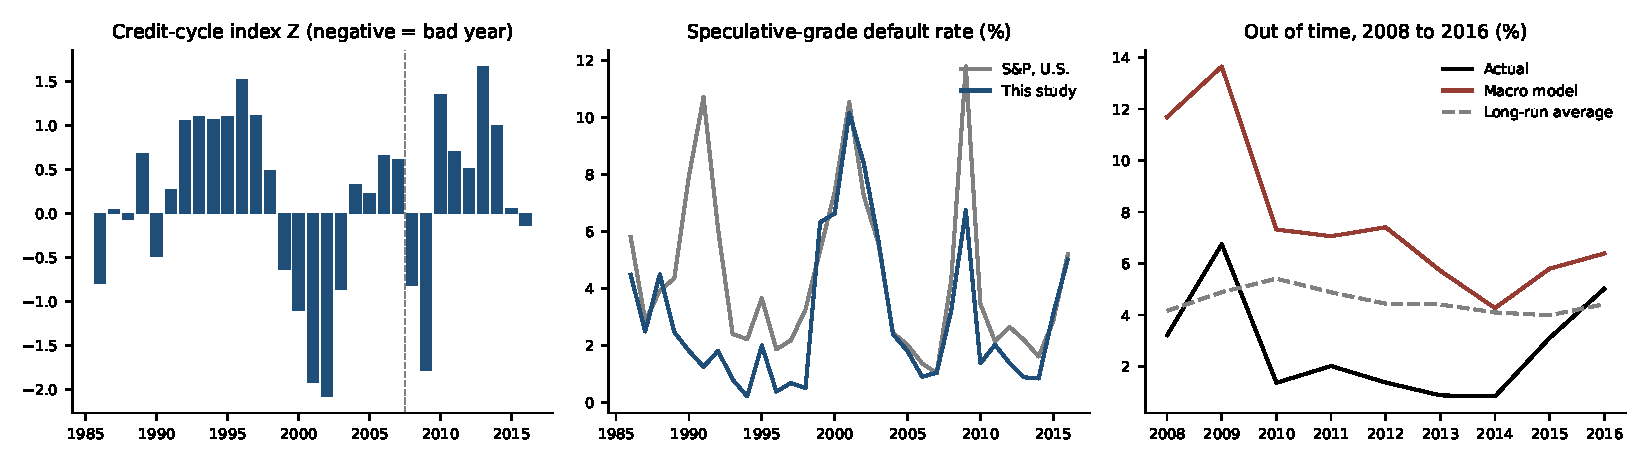
\includegraphics[width=\textwidth]{figure1.pdf}
\caption{Left: fitted cycle index; the dashed line separates estimation and out-of-time years. Middle: default rates in this study against S\&P. Right: out-of-time predictions.}
\end{figure}

\begin{table}[h]
\centering\small
\begin{tabular}{lrr}
\toprule
Mean absolute error, 2008 to 2016 (percentage points) & Against the file & Against S\&P \\
\midrule
Macro model ($Z$ predicted from macro data) & 4.97 & 3.68 \\
Through-the-cycle average & 2.34 & 2.24 \\
Fitted $Z$ (uses that year's migrations; not a forecast) & 1.55 & 1.19 \\
\bottomrule
\end{tabular}
\caption{Out-of-time test. The second column, scored against S\&P's U.S. rates, was not preregistered; it was added after the data check.}
\end{table}

\textbf{H2: fails.} The macro model over-predicts defaults in every year from 2008. Credit spreads stayed wide after the crisis while defaults fell quickly, so the spread-to-cycle relationship fitted before 2007 did not hold. The cycle factor itself carries information (the fitted-$Z$ row beats the average), but macro data did not recover it out of sample.

\textbf{H3: passes on paper, not credible.}

\begin{table}[h]
\centering\small
\begin{tabular}{lrrr}
\toprule
Case & $Z$ & Spec.-grade default rate & BBB to spec. grade or default \\
\midrule
Through-the-cycle average & & 4.42\% & 6.29\% \\
Worst fitted year (2002) & $-2.08$ & 7.69\% & 11.37\% \\
Severely adverse, 2025 & $-7.21$ & 24.94\% & 36.12\% \\
Severely adverse, 2026 & $-5.30$ & 16.91\% & 25.11\% \\
Severely adverse, 2027 & $-2.04$ & 7.62\% & 11.26\% \\
\bottomrule
\end{tabular}
\caption{Stress projection, grade mix of the December 2015 cohort.}
\end{table}

The scenario's spread is 5.24 after bridging the Fed's BBB yield to Baa (+0.64), against a fitted range of 1.51 to 3.19. $Z = -7.2$ is more than three times past the worst fitted year, from a model that already failed out of time. The ratio of 5.65 meets H3 mechanically, but the defensible stress is the worst-fitted-year row, 1.74 times the average. Even that understates real peaks: the actual rate was 10.16\% in 2001.

\textbf{Robustness.} Refitting on the 1998 to 2006 cohorts only ($\rho = 0.033$, $n = 9$) leaves both conclusions unchanged: out-of-time error 4.19 for the macro model against 2.34 for the average, and a severely adverse peak of 20.11\%.

\section{Limits}

\begin{itemize}
\item The ratings file misses defaults before 1999 and some in 2009 to 2014, so default levels are understated in those years.
\item One systematic factor, with no industry or regional factors; it does not capture default peaks fully.
\item The macro regression has 22 annual observations and is driven by one variable.
\item The scenario lies outside the estimation range, so the projection tests the model's extrapolation, not its fit.
\end{itemize}

\section{Reproducibility}

Code and aggregate results: \texttt{src/01} to \texttt{07} and \texttt{results/}. Every number above is printed by a script and recorded in \texttt{RESULTS\_LOG.md}. The ratings data is licensed and is not distributed.

\end{document}
